
\section{Calculating Reputation: Miners and Merkle Proofs}\label{sec:reputationmining}
We see that the reputation system is a core component of any decentralised colony. By carefully balancing the rewards and penalties we aim to keep every users' incentives aligned with the colony and the colony network. Since reputation can only be \emph{earned} and not bought, the system fosters a more meritocratic from of decision making than pure token-weighted voting can hope to achieve. The continuous decay of reputation ensures that the influence conveyed by reputation is recent and up-to-date; it prevents a reputation aristocracy and allows for a fluid passing of control from one set of contributors to another over time.

How well the parameters of the reputation system balance out competing interests will have to be subject to empirical review when the colony network begins live operation and any parameters proposed in this document should be seen as suggestions, not prescriptions for the final network.

Due to the combined complexity of reputation scores across multiple colonies, domains and skills %; growing due to tasks completed and disputes won; shrinking due to decay and poor performance;
\textbf{reputation scores cannot be stored and calculated on-chain}. Instead, the calculations will all take place off-chain, the results of which will be reported to the blockchain by participating CLNY holders --- in a process resembling a proof-of-stake blockchain consensus protocol. We call this procedure \textbf{`Reputation Mining'}.\\
The reputation calculation whose result the miners are submitting, is determined by the activities that have taken place in the colonies and can be fully deterministically derived from the ethereum blockchain. Game-theoretically the system is protected similarly to the off-chain calculations of truebit (\cite{TruebitWhitepaper}) in that, \emph{while the calculation cannot be done on-chain and a correct submission can never be proved true, an incorrect calculation can always be proved to be wrong.}


\subsection{The Reputation Tree and the ReputationRootHash}\label{sec:reptree}
A reputation consists of the following data:
$$
R = 
\begin{cases}
 rep\_id & \textnormal{the id of a skill or domain identifying the type of reputation},\\
 colony\_id & \textnormal{the colony the reputation is held in},\\
 user & \textnormal{the address holding the skill},\\
 amount & \textnormal{the numerical value of the reputation}.
\end{cases}
$$
All individual reputations are assembled into the \textbf{``Reputation Tree''} which is a merkle tree (\cite{MerkleTrees}, \cite{MerkleInEthereum}) of all individual reputations in a colony and the cumulative totals. (Note: The tree also contains the totals of all types of reputation held by users in this colony; these are entries in which the \ascode{user} is set to zero.)\\
All reputations held by all users in all colonies are ordered in a list. The elements of this list are hashes pairwise, to end up with a shorter list of hashes. This process is repeated until only one hash remains: the \ascode{ReputationRootHash}, $\mathcal{RH}$.
\begin{center}
\begin{tikzpicture}
 \node at (0,-5) (r1) {$R_1$};
 \node at (1.5,-5) (r2) {$R_2$};
 \node at (3,-5) (r3) {$R_3$};
 \node at (4.5,-5) (r4) {$R_4$};
 \node at (6,-5) (rdots) {$\cdots$};
 \node at (8,-5) (rn) {$R_N$};
 %
 \node at (0,-4) (r1hash) {$\mathcal{H}(R_1)$}
  edge[-] (r1);
 \node at (1.5,-4) (r2hash) {$\mathcal{H}(R_2)$}
  edge[-] (r2);
 \node at (3,-4) (r3hash) {$\mathcal{H}(R_3)$}
  edge[-] (r3);
 \node at (4.5,-4) (r4hash) {$\mathcal{H}(R_4)$}
  edge[-] (r4);
 \node at (8,-4) (rnhash) {$\mathcal{H}(R_N)$}
  edge[-] (rn);
 %
 \node at (1,-2.5) (r12) {$\mathcal{H}_{1,2}$}
  edge[-] (r1hash)
  edge[-] (r2hash);
 \node at (3.75,-2.5) (r34) {$\mathcal{H}_{3,4}$}
  edge[-] (r3hash)
  edge[-] (r4hash);  
 \node at (7,-2.5) (rnn) {$\mathcal{H}_{N,N-1}$}
  edge[-] (rnhash)
  edge[dashed] (6.5,-4);
 %
 \node at (2.5,-1) (r14) {$\mathcal{H}_{12,34}$}
  edge[-] (r12)
  edge[-] (r34);
 %
 \node[draw, fill=gray!5] at (4,0) (root) {\texttt{ReputationRootHash}};
 \node[right = 2mm of root] (rh) {$\mathcal{RH}$} 
   edge[-] (root);
 \node[below = 1mm of root] (dummy) {\phantom{a}}
  (dummy.north west) edge[dashed] (r14)
  (dummy.north east) edge[dashed] (rnn);
 %
 %
 \node at (4,-6) (label) {\textnormal{The Reputation Tree}};
\end{tikzpicture}
\end{center}

In the event of a starting or an intermediate array being an odd number (which will always happen for a starting array that is not a power of two), the hash contained in the last element is hashed with itself.

The \ascode{ReputationRootHash} is the data we record on the blockchain. It represents an integrity check for the entire reputation system and whenever a user wishes to make use of their reputation, the can submit a merkle proof starting at the reputation $\mathcal{R}_i$ they wish to make use of and ending at $\mathcal{RH}$.

\subsection{Calculating the new root hash}
To calculate the new root hash, the miners begin with the last reputation state, and decays all reputations held by all users in all colonies, in the order of the leaves in the tree. They then take the set of reputation gains or losses due to good or bad behaviour that were not in the last state submitted, and are to be included in the next state. They apply the reputation updates to each user, in each colony, to end up with a new list of reputations for all users and colonies. These new reputations are then hashed and assembled into a new merkle tree yielding an updated \ascode{ReputationRootHash}.

While the calculation is too large to be done on-chain due to technical (gas limit) and economic (gas cost) limitations, it is expected that this calculation can easily be performed by any consumer grade laptop computer.

\subsection{Submission of a new root hash}
%
\subsubsection*{What is submitted?}
The final \ascode{ReputationRootHash} is submitted to the contract by the miner along with the number of leaves in the tree. Further, the miner also submits the IPFS/Swarm hash of a document containing the entire state tree (though this is only for convenience; any user can construct this locally based on the blockchain history).
%
\subsubsection*{Who can submit a new root hash?}
CLNY token holders are eligible to become miners and participate in the reputation update process, but since any user can calculate the correct root hash locally, it would be possible for \emph{any} \rcth to submit the hash to the contract.
It is however undesirable to have too many submissions for every update. We propose a mechanism that only allows some miners to submit results to begin with. To participate in the mining process, \rcths must stake some of their tokens to become `reputation miners'. A submission will only be accepted from a miner if \ascode{SHA3(address, N, hash)} is sufficiently small (\ascode{< target}). At the beginning of the submission window, the target is set to 0 and slowly increases to $2^{256}\times10^{-3}$ after 150 blocks. The fact that the target is capped, rather than increasing to $2^{256}$ at the end of the submission period effectively creates a minimum number of tokens required to submit a hash. This puts a tangible cost on any attacks revolving around spamming known false submissions (see section \ref{}). This factor will be changeable by the \rc.

The variable $N$ that goes into the hash is some number greater than 0 and less than the number of tokens the \rcth address has staked divided by $10^15$, meaning that users with a large stake have a higher chance of qualifying to submit a hash than smaller stake holders. The factor of $10^15$ is introduced to ensure that all hashes a user is eligible to submit can be calculated in a few seconds by the client.
%
\subsubsection*{Verifying a submission}
If only one state is submitted by the end of the submission period, then the new state is accepted, and proposals of the next state can begin to be made. This is expected to be the most common occurrence.\\
If more than one state has been submitted, then either someone has made a mistake, or there is a malicious entity trying to introduce a fraudulent reputation change. In this event, the a challenge-response protocol can establish which state is incorrect (see Section \ref{sec:challengeresponse})

\subsubsection*{Mining Rewards}

When a state is accepted, a small number of (newly generated) \rcts are made available for the user who first submitted the correct state to claim as a reward. When the user claims this payout, they receive a corresponding amount of reputation in the \rc (a special mining skill, which only users in the root colony can earn by performing this task). This reputation update is no different from any other, aside from the limitations of who is able to earn it, and will be included in a subsequent reputation update cycle.

\subsection{Dealing with false submissions}\label{sec:challengeresponse}
The challenge-response mechanism detailed below relies heavily on merkle proofs, so it will be useful to establish some notation.

\subsubsection{Merkle Proofs}
Consider the merkle tree shown in figure below. In order to prove that the element \ascode{A} is in the tree with root \ascode{G}, one submits a merkle proof containing the following information: \ascode{A, [B,F], [l,l]}. The first argument is the element whose existence is to be proved. The second argument is the list of hashes that \ascode{A} should be hashed pairwise with. The last argument is an array of \ascode{l}'s and \ascode{r}'s that indicates whether the hash calculated so far should be hashed on the left or the right of next element in question. So to show that \ascode{C} was in the tree with root \ascode{G}, the proof would be of the form \ascode{C, [D,E], [l,r]}.
\begin{center}
 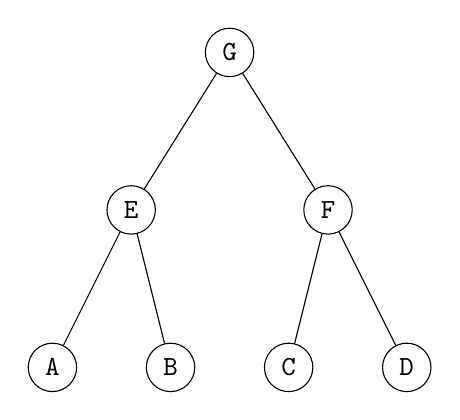
\begin{tikzpicture}
  \node[shape=circle, draw] at (0,-4) (a) {\texttt{A}};
  \node[shape=circle, draw] at (1.5,-4) (b) {\texttt{B}};
  \node[shape=circle, draw] at (3,-4) (c) {\texttt{C}};
  \node[shape=circle, draw] at (4.5,-4) (d) {\texttt{D}};
  %
  \node[shape=circle, draw] at (1,-2) (e) {\texttt{E}}
   edge[-] (a)
   edge[-] (b);
  \node[shape=circle, draw] at (3.5,-2) (f) {\texttt{F}}
   edge[-] (c)
   edge[-] (d);
  %
  \node[shape=circle, draw] at (2.25,0) (g) {\texttt{G}}
   edge[-] (e)
   edge[-] (f);
 \end{tikzpicture}
\end{center}
Note also that the array of \ascode{l}'s and \ascode{r}'s nothing more than a binary representation of the leaf node's index in the tree. When expressed in this way, we refer to the index as the `path' in the merkle proof. We refer to the objects that get hashed along the way (e.g. \ascode{[D,E]}) as the `siblings'.
%
\subsubsection{The Challenge-Response Protocol}
We assume that the correct hash is one of the  submitted hashes. This is a reasonable assumption, as only one out of all the miners is required to make a correct submission, and there is an incentive for them to do so (Section \ref{subsec:mining-costs-and-rewards}). Thus our task is not to validate the correct hash but to invalidate the false ones.

We must prove all but one submission incorrect by having each submission navigate a series of challenges. These \emph{challenges} refer to events that happened in the colony network within the last update cycle that have a reputation effect while the \emph{responses} to the challenges are merkle proofs that the corresponding reputation update was properly handled.

\subsubsection*{1. The Justification Tree}
 The first step is for both parties to upload a second merkle root. This is the root of a tree where each leaf represents a complete reputation state i.e. each leaf is a \ascode{ReputationRootHash}. The right-most leaf ($\mathcal{RH}_n$) is the hash they originally submitted, the left-most leaf ($\mathcal{RH}_0$) is the final accepted reputation state from the last update, and the intermediate leaves ($\mathcal{RH}_i$) represent the evolution of the reputation state after the reputation updates are applied one-at-a-time. 
 %
 \newcommand{\jrh}{\ensuremath{\mathbb{JRH}}}
 %
\begin{center}
\begin{tikzpicture}
 \node at (0,-4) (rh0) {$\mathcal{RH}_0$};
 \node at (1.5,-4) (rh1) {$\mathcal{RH}_1$};
 \node at (3,-4) (rh2) {$\mathcal{RH}_2$};
 \node at (4.5,-4) (rh3) {$\mathcal{RH}_3$};
 \node at (6,-4) (rh4) {$\mathcal{RH}_4$};
 \node at (7.5,-4) (rdots) {$\cdots$};
 \node at (9.5,-4) (rhn) {$\mathcal{RH}_n$};
 %
 \node at (0.75,-2.5) (rh01) {$j_{01}$}
  edge[-] (rh0)
  edge[-] (rh1);
 %
 \node at (2.25,-2.5) (rh12) {$j_{12}$}
  edge[-] (rh1)
  edge[-] (rh2);
 %
 \node at (3.75,-2.5) (rh23) {$j_{23}$}
  edge[-] (rh2)
  edge[-] (rh3);  
 %
 \node at (5.25,-2.5) (rh34) {$j_{34}$}
  edge[-] (rh3)
  edge[-] (rh4);  
 %
 \node at (8.5,-2.5) (rhnn) {$j_{n,n-1}$}
  edge[-] (rhn)
  edge[dashed] (8,-4);
 %
 \node at (1.75,-1) (rh02) {$j_{02}$}
  edge[-] (rh01)
  edge[-] (rh12);
 %
 \node at (4.5,-1) (rh24) {$j_{24}$}
  edge[-] (rh23)
  edge[-] (rh34);
 %
 \node at (3.7,0) (dummy14) {$j_{04}$}
  edge[dashed] (rh02)
  edge[dashed] (rh24);
 %
 \node[draw, fill=gray!5] at (5,1) (root) {\texttt{JustificationRootHash}};
 \node[right = 2mm of root] (jrh) {$\jrh$} 
   edge[-] (root);
 \node[below = 1mm of root] (dummy) {\phantom{a}}
  (dummy.north west) edge[dashed] (dummy14)
  (dummy.north east) edge[dashed] (rhnn);
 %
 %
 \node at (4,-5) (label) {\textnormal{The Justification Tree}};
\end{tikzpicture}
\end{center}
Note that in the first stage of the tree, every neighnouring pair of leaves is hashed, and so any pair has a shared merkle proof to the root.\\
Any two differing submitted states agree on the first leaf $\mathcal{RH}_0$ (the \ascode{ReputationRootHash} accepted at the end of the previous iteration of the mining process), and disagree on the last leaf $\mathcal{RH}_n$. Somewhere there is a transition  ($\mathcal{RH}_i$ to $\mathcal{RH}_{i+1}$) where they agree on the starting state but disagree on the result. This transition is meant to be the effect of a single reputation update, the calculation of which is able to be done on-chain. \\
First, however, we must establish where the two overall calculations submitted differ.

\subsubsection*{2. Searching for the discrepancy}
The contract requires both parties to submit merkle proofs that specific reputation updates were handled correctly. It begins by pseudorandomly picking a reputation updating transaction from the first half of the log (Appendix \ref{appendix:rep-transfer}) (say the $i^{th}$ update for some $i<\frac{n}{2}$) and requires both parties to provide:\\
\begin{itemize}
 \item[(i)] The root hash before the update was applied ($\mathcal{RH}_{i-1}$)
 \item[(ii)] The root hash after the update was applied ($\mathcal{RH}_i$)
 \item[(iii)] A merkle proof showing that the pair ($\mathcal{RH}_{i-1}, \mathcal{RH}_i$) is correctly included in the justification tree
\end{itemize}

The contract then repeats this process using a binary search algorithm. If the merkle proof (iii) for both submissions had the same sibling values almost all the way up, but differing only in the the final sibling, then the discrepancy must occur later (i.e. the two sumbissions differ at some $i^\prime > \frac{n}{2}$) whereas if the merkle proofs already differ at an earlier sibling, then the submissions must also differ in an update before $\frac{n}{2}$. This final hash is stored as the new target hash for following challenges.

The contract pseudorandomly selects a reputation update from within the subtree in which the first discrepancy is known to lie. Each newly submitted proof further reduces the size of the subtree by a factor of two\footnote{ By examing precisely at which sibling the first discrepancy occurs, some stages of the binary search could be skipped. However, in order to accomplish this all the siblings of the proof that first completed the challenge would need to be stored on the blockchain, so it’s likely that it is more gas efficient to just do the `naive' binary search.}.

If at any point in the process, a submission does not respond to the challenge, in a timely fashion they forfeit, and are assumed to be incorrect. If all submissions continue to be defended successfully, ultimately, the location of the first discrepancy in the series of state transitions is found: the submissions aggree on (i) but not (ii). The contract then requires
\begin{itemize}
 \item[(iv)] A merkle proof for the reputation ($R_j$) affected by the $i^{th}$ update trasaction.
\end{itemize}
Note: in point (iv), the \emph{exact same} merkle proof that proves the inclusion of $R_j$ (before the reputation update) in the root $\mathcal{RH}_{i-1}$ must also prove the inclusion of $R_j$ (after the reputation update) in the root $\mathcal{RH}_i$. This is because the trees $\mathcal{RH}_{i-1}$ and $\mathcal{RH}_i$ differ in only a single leaf.\\

Finally, this transition is then calculated on-chain to determine which is the correct answer. The submission that has been proved to be incorrect is rejected.

In the event of more than two submissions, this process is conducted in parallel between multiple pairs of submitted hashes, and then repeated, until only one submission remains.

If less than an hour elapses from submissions opening to only one submission remaining, the next submission window only opens when a hour has passed from the start of this window. If more than an hour has passed, the next submission window opens immediately.



\subsection{Implementation Details}
%
\subsubsection{Keeping track of reputation changes}
%
There are two types of reputation update that occur:
\begin{itemize}
 \item Decay of existing reputation
 \item Addition or removal of reputation as a reward or punishment.
\end{itemize}
All reputation decays, and so it is only the latter that is explicitly recorded on the blockchain when an event occurs. Specifically, when a reputation affecting event occurs, an entry is added to the `reputation update log' in the \rc. Such an entry consists of
\begin{center}
\begin{tabular}{lll}
$R$ &--& The reputation to be updated\\
$\Delta_R$ &--& The reputation change\\
source &--& An address if the reputation is coming from someone, zero otherwise\\
$n\_updates$ &--& The cumulative number of all reputation changes that will have been made\\
	    & & when this log entry is correctly processed.\\
\end{tabular}
\end{center}

Recall also from section \ref{sec:reptree} that a reputation consists of
\begin{center}
\[
R = 
\begin{cases}
 rep\_id & \textnormal{the id of a skill or domain identifying the type of reputation},\\
 colony\_id & \textnormal{the colony the reputation is held in},\\
 user & \textnormal{the address holding the skill},\\
 amount & \textnormal{the numerical value of the reputation}.
\end{cases}
\]
\end{center}

%I suggest we do a little appendix of data structures. That way we can refer to reputations and rep_ids an other data here without having to fully document it here. We would not need to even mention the parent_id and parent_n_id here (as we need it onle elsewhere)...

Furthermore for each $rep\_id$, the following data is also known
\[
  rep\_id \rightarrow 
  \begin{cases}
    parent\_id &	\textnormal{the rep\_id of the parent domain/skill}\\
    parent\_n\_id &	\textnormal{the rep\_id of the $n^{th}$ parent}\\
    generation &	\textnormal{total number of parents}\\
    children\left[\cdots\right] &	\textnormal{array of children}\\
    n\_children &	\textnormal{total number of children}
  \end{cases}
\]
When a user earns reputation in a skill or domain, s/he also earns reputation in all parents and thus corresponds to \ascode{generation+1} number of reputation updates. Alternately, when a user loses reputation, they also lose reputation in all parents and all children representing a total number of updates of \ascode{generation + n\_children + 1}. (Note: parent\_id and parent\_n\_id are not used here; they are used during dispute escalation - see Section \ref{sec:disputes}).

It is only by recording the number of parent reputations (\ascode{generation}) and how many reputations have been updated already in this update cycle (via \ascode{n\_updates}) that the resolution protocol is able to perform the binary search of the justification state trees submitted by the disagreeing users. At the start of the challenge protocol, the contract can look up the last entry in the update table for the cycle under consideration, and work out how many updates have occurred in this cycle based on the number of updates prior and the number of parent reputations. It can then conduct the binary search.

When the discrepant state transition is found, the users supply the index of the update on-chain that corresponds to that reputation update. This means that the contract does not have to iterate over the whole list expensively, but the contract can easily check the correct reputation update is being considered, and then confirm that the calculation made corresponds to the correct reputation update. In the event that the discrepant transaction is a decay transaction, which is easily determined by the merkle path corresponding to an index smaller than the number of leaves in the tree at the end of the last successful update, they must also supply a merkle proof that the starting value assumed for the user corresponds to the value that user had at the end of the last update cycle.

Recording the number of leaves in the tree is required to allow the binary search to occur and accommodate the decay calculations that must be done at the start of each update. Before any new reputation is earned or lost in an update cycle, all existing reputations owned by users decays (see next section \ref{sec:repdecay}). There is a decay calculation for every leaf in the previously accepted tree. We do the decay calculations first to give users the benefit of the doubt during reputation updates so they do not lose reputation they have only just earned to premature decay.

When a user earns reputation in a new skill, at least one new leaf is added to the tree - if they have not earned reputation before in some of the parents, then they will also cause further new leaves to be added. New leaves will also be added if they are the first user in a colony to earn those particular skills, making the total reputation for that skill in the colony non-zero. During a dispute, when the user proves that they have included the update in the tree, it is not possible to check (efficiently) on-chain that they should not have added it to an existing leaf instead. However, because during a dispute we are always playing two submissions off against the other, one of two things will be true:
\begin{itemize}
 \item Both submissions add a new leaf to the tree. If there was a discrepancy, then it is in the maths conducted on this leaf, not the addition of the leaf itself. The maths can be checked on-chain to establish which result is correct.
 \item The other submission adds the new reputation to an existing leaf (the correctness of which can be checked on-chain easily). In this case, the user who added the leaf incorrectly is wrong.
\end{itemize}





\subsubsection{Transfers of reputation between accounts}\label{sec:reptransfer}

The most important quality of reputation that distinguishes it from a token is that it is tied to an account and cannot be transferred. However, in the event of disputes (Section \ref{sec:disputes}) it can happen that one party to a dispute loses reputation while the other gains. This process has to be modelled as a `reputation transfer' to ensure that reputation is never created in this process (i.e. the reputation lost by the loser is at least as much as the reputation gained by the winner).

If an entry in the reputation update log indicates that the reputation has come from another user, then this entry represents updates of all the parents of the reputation being gained by one user, and updates of all the parents and children of the reputation being lost by the other. However, we have to ensure that the user who is losing reputation still has the reputation to lose if another user is gaining it.

To achieve this, all the transactions that correspond to updating the reputations of the user gaining the reputation are done first. In the event such a transaction must be proved to be correct in the resolution protocol, the users can provide a proof of the losing user’s reputation, prior to them losing it in this update, and this can be compared to the amount of reputation intended to be gained. Whichever is smaller is used as the amount of reputation the user is gaining during the calculations.

Then, when calculating the reputation deduction to be applied to the losing user, the reputation that was used for as the voting weight should be done last i.e. all the children (and parents) should be considered first, as it is the amount of the reputation that was eligible to vote that will determine the fraction lost of each of the children reputation. %If any of these calculations need to be proved correct during the resolution protocol, 

For further details about reputation transfers and disputes, see Appendix \ref{appendix:rep-transfer}.

\subsubsection{The Reputation Decay Process}\label{sec:repdecay}
The reputation decay process was describe above as being continuous. To have a user's reputation continuously decay, and end up with half of the starting amount after three months, an exponential decay makes most sense. However, such a calculation is not possible on-chain, so we must use an approximation. The details of the approximation we use, and a proof that this approximation is accurate and will not affect the running of (active) colonies can be found in appendix \ref{appendix:rep-decay}.


\subsection{Possible Attacks}
\subsubsection*{Many false submissions}
% If we cannot figure out what the correct submission is within the given timeframe, then the reputation update process stalls... that's about it though. Very expensive attack and only effect is to delay one update.
In the event of multiple submissions, finding the correct one takes time --- the timeout $t$ for the challenge-response must be reasonable to allow the transaction defending a submission to propagate and be mined. A denial-of-service attack is therefore possible, whereby an attacker makes many false submissions. However, if these submissions were random hashes, unable to be defended, then none would be defended correctly within the first five minute window, and the attack would quickly end. 

The denial of service attack can only be sustained when the false submissions are incorrect only in some leaves, and the majority of the state tree is correct. In this scenario, the attacker successfully defends each of their submissions for as long as possible to delay the resolution of the reputation mining protocol as much as possible.

Any such attack is capped by the first round of pairings of submissions against each other. Even if the attacker made millions of submissions, only a finite number of those would be able to be successfully defended due to the block size --- currently, no more than 4500 submissions would be able to be defended, even if the attacker used up all block space during the timeout.\footnote{These figures assume $1.5\pi\times10^6$ gas in a block, and that each transaction is only 21000 gas for a worst-case-scenario calculation. In reality the transactions would be larger, and the attacker is unlikely to be able to exclusively fill every block. Furthermore, even though the attacker is filling the blocks with their transactions, we assume that the defense of the legitimate state is always successfully included in block, as a one-off increase in gas costs will always be worthwhile to ensure the legitimate state is defended. } With only 4500 submissions able to make it to the second round, the length of time the DoS attack would be sustained for is given by 

$$t \times \left\lceil\log_2\left(4500\right)\right\rceil\times \left\lceil\log_2\left(N_{\rm updates}\right)\right\rceil$$

\noindent where $N_{\rm updates}$ is the number of reputation updates that have been made in this update cycle. To arrive at this figure, we know there will need to be $\left\lceil\log_2\left(4500\right)\right\rceil$ rounds of comparison between submissions to eliminate all but one. Each round will require $\left\lceil\log_2\left(N_{\rm updates}\right)\right\rceil$ interrogations of the justification tree to establish where the two submissions being compared differ. Finally, each interrogation can take up to $t$ before it is considered to have timed out and one or both of the submissions is deemed invalid. The product of these three factors tells us how long this reputation update can be delayed by an attacker.

Long term, $N_{\rm updates}$ will be dominated by the decay transactions rather than by any updates that have occurred since the last reputation state was established. Even if the Colony Network were wildly successful, with 100000 colonies, each with 1000 users that had earned some reputation in 1000 different skills in each of the structural and skill hierarchies, the delay to the reputation updates would only be around $36$ hours.

There would be little effect on the rest of the colony network in this time. Users would still be able to exercise their reputation from the previous reputation update, and continue to influence decisions with that reputation. Indeed, this shows what perhaps the main motivation for such an attack would be --- if a user knew that they had been `caught' behaving badly, and was due to lose all their reputation, they might try such an attack to eke out the last bits of influence they possibly could. However, decisions in the colony network do not resolve quickly, and in a well-developed colony we would not expect any one person to have a large amount of reputation when compared to the rest of the colony, so it seems unlikely they would be able to unduly influence decisions significantly while conducting the attack.

Assuming this attack continued, then the reputation mining protocol would effectively only update every 36 hours. Users staking would become more susceptible to variance in terms of the rewards, but otherwise little would change in the day-to-day functioning of any individual colony. 

The attacker would lose all the \rct that they had staked (which would be around 4500 times the expected minimum stake) in order to perform the attack, and so would have to buy more to attack again.

\subsection{Costs and Rewards of Mining}\label{subsec:mining-costs-and-rewards}
In order to be involved in the reputation mining process, \rcths must stake their tokens with the Colony Network Contract. This allows them to submit a reputation hash as part of the reputation mining process described above.

If they submit a new hash, this is recorded and they are noted as the first address to submit that hash. If they submit a hash that has already been submitted, they are appended to a list of users that have submitted that hash.

If a hash is found to be incorrect, all those who submitted it lose their stake. If a hash is found to be correct, however, the users who submitted it gain root colony tokens and reputation. The total amount of reputation earned is controlled by the amount of reputation that exists in the colony, and tries to ensure that 25\% of the reputation in a colony comes from mining. If normal activity in a colony generates $A$ reputation per hour, the total reputation that exists $R$ is given by 

$$\frac{A}{1-\exp\left(-k\right)}$$

\noindent On where $k$ is the decay constant used in each update period (see appendix \ref{}). If we wish for 25\% of $R$ to come from mining, then the amount of reputation earned from mining in each update period should be 

$$\frac{R}{4}\left(1-\exp\left(-k\right)\right).$$

When a user makes their submission, their weighting for that hash is recorded, and the total weight submitted by all users for that hash is updated. A staker's weight is given by 

\begin{equation}\label{eq:stakerweight}
\left(1-\exp\left(-\frac{t}{T}\right)\right) \times \frac{1}{n+S} \times B
\end{equation}

where $B$ is the total number of tokens they have staked, $n$ is their position in the list, $S$ and $T$ are normalising constants, and $t$ is the number of blocks they have staked their tokens for. 

The first factor in equation \ref{eq:stakerweight} encourages users to stake their tokens for long periods of time. After $T$ blocks, this first factor is 0.63 of what it will eventually grow to given unlimited time. We expect $T$ to represent around a month.

The second factor in equation \ref{eq:stakerweight} encourages users to submit the hash as soon as possible, with this factor becoming smaller the later users submit; the first submission will have approximately twice the weight of the last submission, all other factors being equal. This factor also means that users are not incentivised to split up their holdings, as some of the split up tokens will have lower weightings. $S$ should be a number on the order of the number of people that are staking in each round to ensure the discrepancy between the rewards for being first and last are not huge; it should be under the control of the \rc.

The last factor $B$ is the number of tokens the user has staked --- if they have staked more tokens, they get more of the payout than they would have done if they had staked less.


FIXME\\
Notes:\\
-token holders must stake in order to be miners\\
-reputational reward comes from tokens earned just like task payout
-how much rep exactly you get (similar to 5 star rating for work) determined by how long you lock your tokens. Short term = 3 stars, long term 5 stars.\\
-how many tokens are paid out to miners must vary as the price of the token changes. Idea: make it scale with the total paid out in other domains of root colony. If feasible, use one month rolling average. Prevent miners overpowering rest of root colony with too much reputation.
- $k$ should be multiplied by the number of hours since the last update to accommodate for attack
- Merkle proof of current $R$ should be submitted with hash, otherwise not accessible on-chain?
